\setcounter{page}{3}
\chapter{Теоретическая часть}
\section{Синтаксическая форма и хранение программы в памяти.}
В $Lisp$ программа синтаксически представлена в форме $S$-выражений. Реализована \textbf{единая форма фиксации}, то есть отсутствие разделения на программу и данные. И программа, и данные представляются списочной структурой. Благодаря такому подходу возможно изменение кода программы при обработке данных. Программа будто может "изменять саму себя".
Так как программа имеет вид $S$-выражения, в памяти она представлена либо как атом (5 указателей, которыми представляется атом в памяти), либо как списковая ячейка (2 указателя, бинарный узел).

\begin{table}[h!]
  \centering
  \begin{tabular}{p{1\linewidth}}
    \centering
    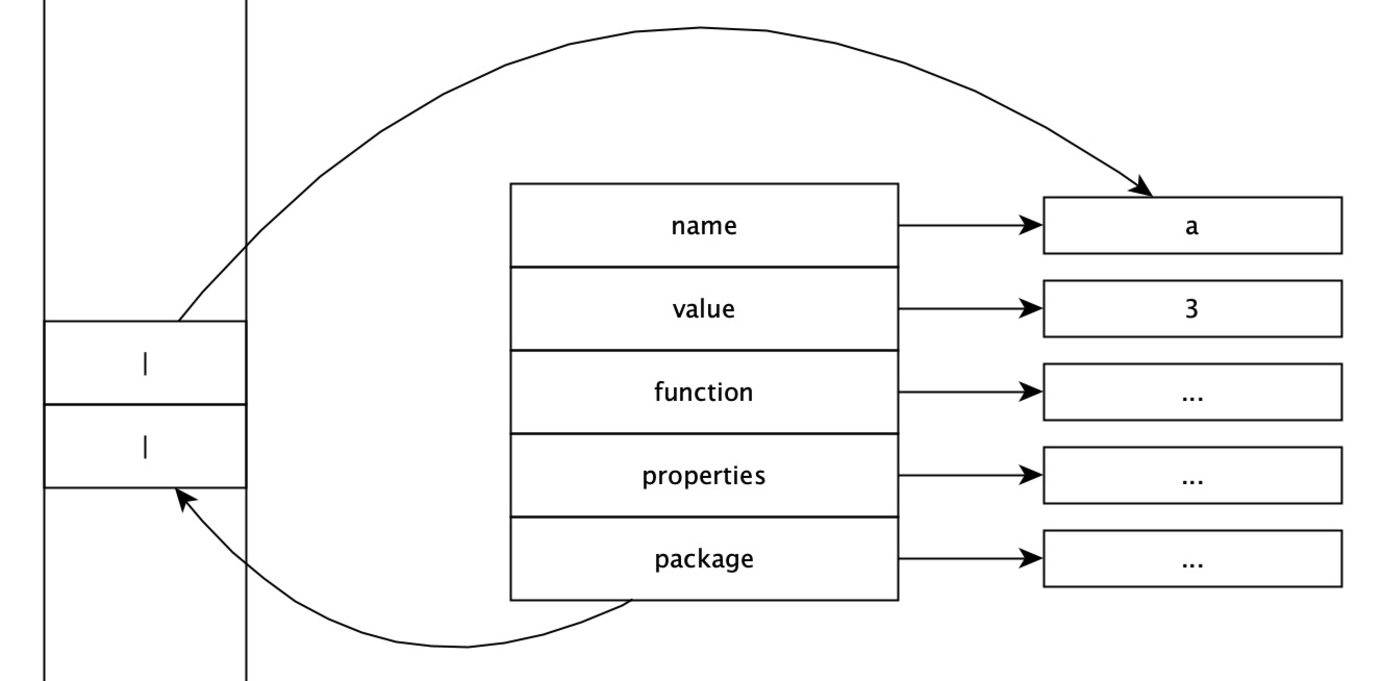
\includegraphics[width=0.7\linewidth]{./images/a.pdf}
    \captionof{figure}{Атом в памяти}
    \label{img:3}
  \end{tabular}
\end{table}

\begin{table}[h!]
  \centering
  \begin{tabular}{p{1\linewidth}}
    \centering
    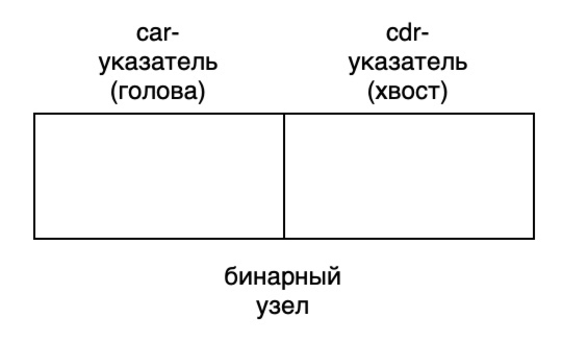
\includegraphics[width=0.3\linewidth]{./images/b.pdf}
    \captionof{figure}{Списковая ячейка}
    \label{img:3}
  \end{tabular}
\end{table}

\section{Трактовка элементов списка.}
При обработке списков первый элемент воспринимается интерпретатором как название функции, все остальные~---~ее аргументы (список трактуется как вычислимая форма). Количество элементов, не считая первого~---~названия функции, должно совпадать с количеством входных аргументов указанной функции.

В случае если перед скобкой применяется блокировка вычислений (' или $quota$), результатом является все, что стоит после блокировки.

\begin{code}
\begin{minted}{lisp}
[2]> (cons 1 2)
(1 . 2)
[3]> (cons 1 2 3)
*** - EVAL: too many arguments given to CONS: (CONS 1 2 3)
[4]> `(cons 1 2)
(CONS 1 2)
\end{minted}
\end{code}

\section{Порядок реализации программы.}
Общий алгоритм:
\begin{enumerate}
	\item Ожидает ввода $S$-выражения.
	\item Передает введенное $S$-выражение функции $eval$.
	\item Выводит полученный результат.
\end{enumerate}

\begin{table}[h!]
  \centering
  \begin{tabular}{p{1\linewidth}}
    \centering
    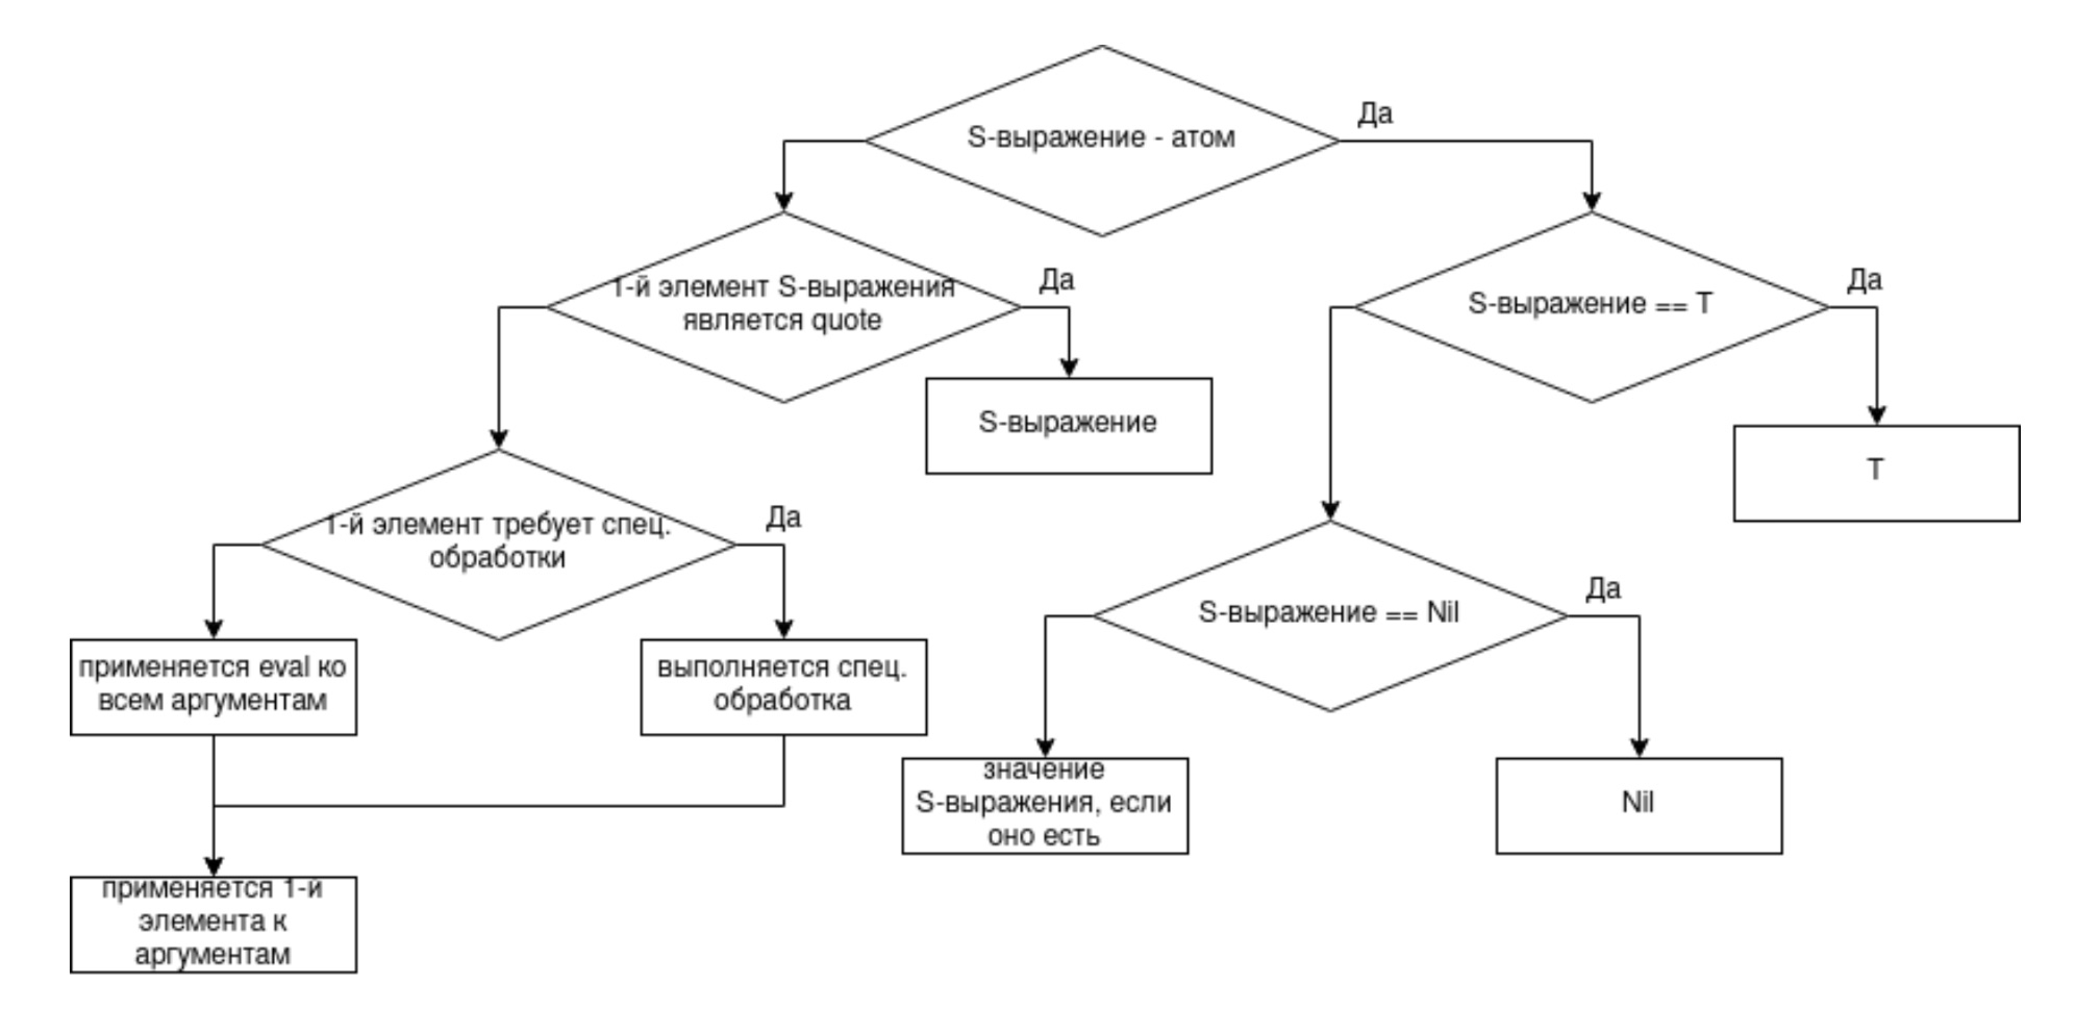
\includegraphics[width=0.67\linewidth]{./images/eval.pdf}
    \captionof{figure}{Диаграмма работы $eval$}
    \label{img:3}
  \end{tabular}
\end{table}

\section{Способы определения функций.}
Функцию можно определить двумя способами: неименованную с помощью $lambda$ и именованную с помощью $defun$.

\begin{equation}
	\nonumber (lambda \quad (x_1 \quad x_2 \quad ... \quad x_n) \quad f),
\end{equation}
где $f$~---~тело функции, $x_i, i = \overline{1, n}$~---~формальные параметры.

\begin{equation}
	\nonumber (defun \quad <\text{имя}> \quad [lambda] \quad (x_1 \quad x_2 \quad ... \quad x_n) \quad f),
\end{equation}
где $f$~---~тело функции, $x_i, i = \overline{1, n}$~---~формальные параметры. Тогда имя будет ссылкой на описание функции.


\section{Работа со списками.}

Ниже перечислены наиболее часто используемые для работы со списками функции.

\subsection{Создание.}
Список можно создать несколькими способами. Базисная функция $cons$ может создавать список, если её второй аргумент является списком.
 
\begin{code}
\begin{minted}{lisp}
[2]> (cons 1 `(2 3 4))
(1 2 3 4)
\end{minted}
\end{code}

Функция $list$ также создаёт список, принимая на вход неопределённое количество аргументов.

\begin{code}
\begin{minted}{lisp}
[3]> (list 1 `(2 3 4) 5 6)
(1 (2 3 4) 5 6)
\end{minted}
\end{code}

Функция $last$ возвращает список, содержащий последний элемент в списке.

\begin{code}
\begin{minted}{lisp}
[4]> (last `(1 2 3))
(3)
\end{minted}
\end{code}

$append$ принимает произвольное количество аргументов-списков и соединяет элементы верхнего уровня всех списков в один список. В результате должен быть построен новый список.

\begin{code}
\begin{minted}{lisp}
[5]> (setf a (list 1 2))
(1 2)
[6]> (append a (list 3 4))
(1 2 3 4)
[7]> a
(1 2)
\end{minted}
\end{code}

\subsection{Изменение.}

Следующие функции будут рассмотрены, применяясь последовательно на примере:
\begin{code}
\begin{minted}{lisp}
[4]> (setf a (list 1 2))
(1 2)
[5]> a
(1 2)
\end{minted}
\end{code}

Конкатенация~---~$nconc$. Похожа на $append$, но в отличие от неё "ломает" свои аргументы, не создавая копии списковых ячеек.

\begin{code}
\begin{minted}{lisp}
[8]> (nconc a (list 3 4))
(1 2 3 4)
[9]> a
(1 2 3 4)
\end{minted}
\end{code}

$reverse$~---~выполняет разворот списка по верхнему уровню списковых ячеек. Создает копию, не "ломая" аргумент. $nreverse$~---~работает аналогично, но без создания копий.

\begin{code}
\begin{minted}{lisp}
[11]> (reverse a)
(4 3 2 1)
[12]> a
(1 2 3 4)

[13]> (nreverse a)
(4 3 2 1)
[14]> a
(4 3 2 1)
\end{minted}
\end{code}

\subsection{Селекторы.}
Функция $car$ используется для получения $car$-указателя~---~указателя на голову списка. Функция $cdr$ используется для получения $cdr$-указателя~---~указателя на хвост списка.

\begin{code}
\begin{minted}{lisp}
[6]> (car '(1 2 3 4))
1
[7]> (cdr '(1 2 3 4))
(2 3 4)
\end{minted}
\end{code}

Также, можно использовать композицию функций.

\begin{code}
\begin{minted}{lisp}
[8]> (caddr '(1 2 3 4))
3
[9]> (caadr '(1 (2 5) 3 4))
2
\end{minted}
\end{code}

\newpage

\chapter{Практическая часть}
\section{Задание №1}
\subsubsection{Теория}
\textbf{Чем принципиально отличаются функции cons, list, append?}

Функция $cons$ принимает 2 указателя на любые $S$-выражения и возвращает новую списковую ячейку, содержащую 2 значения. Если второе из переданных значений~---~атом, то создаётся точечная пара. Иначе эта функция включает значение первого аргумента в начало списка, являющегося значением второго аргумента. Следующие две функции определяются с помощью $cons$.

Функция $list$ составляет список из значений своих аргументов, создавая столько списковых ячеек, сколько аргументов ей было передано и расставляя указатели. У итогового списка голова~---~это первый аргумент, хвост~---~все остальные. Эта функция относится к особым, поскольку у неё может быть произвольное число аргументов, но при этом все аргументы вычисляются.

Функция $append$ принимает произвольное количество аргументов-списков и соединяет элементы верхнего уровня всех списков в один список. В результате должен быть построен новый список. Для всех аргументов, кроме последнего, создаются новые списковые ячейки, таким образом исходных данные не "ломаются". Но при изменении списка, являвшегося последним аргументом функции $append$, список-результат работы этой функции будет изменён.

Обобщая: 
\begin{enumerate}
	\item $cons$ является базисной, $list$ и $append$~---~формы;
	\item $list$ и $append$ принимают произвольное количество аргументов, $cons$~---~фиксированное;
	\item $cons$ создает точечную пару или список, $list$ и $append$~---~список;
	\item $cons$ и $list$ создают новые списковые ячейки для каждого аргумента, а $append$ имеет общие списковые ячейки с последним аргументом-списком.
\end{enumerate}

\subsubsection{Практика}
Пусть $(setf \quad  lst1 \quad '(a \quad b \quad c))$ и $(setf \quad lst2 \quad '(d \quad e))$.
Каковы результаты вычисления следующих выражений?
\begin{enumerate}
	\item $(cons \quad lstl \quad lst2)$
	\item $(list \quad lst1 \quad lst2)$
	\item $(append \quad lst1 \quad lst2)$
\end{enumerate}
  
\begin{code}
\caption{Задание №1}
\label{code:bf2}
\begin{minted}{lisp}
[4]> (cons lst1 lst2)
((A B C) D E)

[5]> (list lst1 lst2)
((A B C) (D E))

[6]> (append lst1 lst2)
(A B C D E)
\end{minted}
\end{code}

\section{Задание №2}
Каковы результаты вычисления следующих выражений, и почему?
\begin{enumerate}
	\item $(reverse \quad '(a \quad b \quad c))$;
	\item $(reverse \quad '(a \quad b \quad (c \quad (d))))$;
	\item $(reverse \quad '(a))$;
	\item $(reverse \quad ())$;
	\item $(reverse \quad '((a \quad b \quad c)))$;
	\item $(last \quad '(a \quad b \quad c))$;
	\item $(last \quad '(a))$;
	\item $(last \quad '((a \quad b \quad c)))$;
	\item $(last \quad '(a \quad b \quad (c)))$;
	\item $(last \quad ())$.
\end{enumerate}

\begin{code}
\caption{Задание №2}
\label{code:bf2}
\begin{minted}{lisp}
[1]> (reverse '(a b c))
(C B A) ; создаёт новый список-копию с обратным порядком элементов

[2]> (reverse '(a b (c (d))))
((C (D)) B A) ; работает на верхнем уровне списковых ячеек

[3]> (reverse '(a))
(A) ; если в списке 1 элемент, результат - копия исходного

[4]> (reverse ())
NIL ; если список пустой, результат - пустой список

[5]> (reverse '((a b c)))
((A B C)) ; работает на верхнем уровне списковых ячеек

[6]> (last '(a b c))
(C) ; создаёт список, элемент которого - последний элемент исходного

[7]> (last '(a))
(A) ; если в списке 1 элемент, результат - копия исходного

[8]> (last '((a b c)))
((A B C)) ; работает на верхнем уровне списковых ячеек
; + если в списке 1 элемент, результат - копия исходного

[9]> (last '(a b (c)))
((C)) ; работает на верхнем уровне списковых ячеек

[10]> (last ())
NIL ; если список пустой, результат - пустой список
\end{minted}
\end{code}

\section{Задание №3}
Написать, по крайней мере, два варианта функции, которая возвращает последний элемент своего списка-аргумента.

\begin{code}
\caption{Задание №3}
\label{code:bf3}
\begin{minted}{lisp}
[11]> (defun get_last (x) (car (last x)))
GET_LAST
[12]> (get_last '(1 2 3))
3
[14]> (get_last '(a d (f e)))
(F E)
[23]> (get_last ())
NIL

[15]> (defun get_last2 (x) (car (reverse x)))
GET_LAST2
[16]> (get_last2 '(1 2 3))
3
[18]> (get_last2 '(a d (f e)))
(F E)
[24]> (get_last2 ())
NIL

[19]> (defun get_last3 (x) (if (<= (length x) 1) (car x) 
(get_last3 (cdr x))))
GET_LAST3
[20]> (get_last3 '(1 2 3))
3
[22]> (get_last3 '(a d (f e)))
(F E)
[25]> (get_last3 ())
NIL
\end{minted}
\end{code}

\section{Задание №4}
Написать, по крайней мере, два варианта функции, которая возвращает свой список аргумент без последнего элемента.

\begin{code}
\caption{Задание №4}
\label{code:bf4}
\begin{minted}{lisp}
[31]> (defun drop_last (x) (reverse (cdr (reverse x))))
DROP_LAST
[32]> (drop_last '(1 2 3))
(1 2)
[33]> (drop_last '(a (b c) d))
(A (B C))
[34]> (drop_last ())
NIL

[57]> (defun drop_last2 (x)
    (if (<= (length x) 1)
        nil
        (or
            (setf (cdr (nthcdr (- (length x) 2) x)) nil)
            x
        )
    )
)
DROP_LAST2
[58]> (drop_last2 '(1 2 (3 4)))
(1 2)
[59]> (drop_last2 '(a b c))
(A B)
[60]> (drop_last2 ())
NIL
\end{minted}
\end{code}

\section{Задание №5}
Напишите функцию $swap-first-last$, которая переставляет в списке- аргументе первый и последний элементы.

\begin{code}
\caption{Задание №5}
\label{code:bf5}
\begin{minted}{lisp}
[1]> (defun drop_last (x) (reverse (cdr (reverse x))))
DROP_LAST
[2]> (defun swap_first_last (x) (append (last x) (cdr (drop_last x)) 
(list (car x))))
SWAP_FIRST_LAST
[3]> (swap_first_last `(1 2 3 4 5))
(5 2 3 4 1)
[4]> (swap_first_last `(1 2 (3 4) 5 ()))
(NIL 2 (3 4) 5 1)
[5]> (swap_first_last `(1 2 (3 4) 5 (a d)))
((A D) 2 (3 4) 5 1)
\end{minted}
\end{code}

\section{Задание №6}
Написать простой вариант игры в кости, в котором бросаются две правильные кости. Если сумма выпавших очков равна 7 или 11~---~выигрыш, если выпало (1,1) или (6,6)~---~игрок имеет право снова бросить кости, во всех остальных случаях ход переходит ко второму игроку, но запоминается сумма выпавших очков. Если второй игрок не выигрывает абсолютно, то выигрывает тот игрок, у которого больше очков. Результат игры и значения выпавших костей выводить на экран с помощью функции $print$.

\begin{code}
\caption{Задание №6 - решение}
\label{code:bf4}
\begin{minted}{lisp}
(defun random_dice ()
	(+ (random 6) 1)
)

(defun random_dice_pair ()
	(cons (random_dice) (random_dice))
)
\end{minted}
\end{code}

\begin{code}
\caption{Задание №6 - решение}
\label{code:bf4}
\begin{minted}{lisp}
(defun play_dice (player) 
	(let ((result (random_dice_pair))) 
		(print (list player 'dice  'is result))
		(if (or (equal result (cons 6 6)) (equal result (cons 1 1)))
			(play_dice player)
			(+ (car result) (cdr result))
		)
	)
)

(defun absolute_win (dice_s)
	(or (= dice_s 7) (= dice_s 11))
)

(defun play_game ()
	(let ((result1 (play_dice 1)))
		(if (absolute_win result1)
			(print "player 1 absolutely won")
			(let ((result2 (play_dice 2)))
				(if (absolute_win result2)
					(print "player 2 absolutely won")
					(cond 
						((< result1 result2) 
						(print "player 2 won"))
						((> result1 result2) 
						(print "player 1 won"))
						(t (print "draw"))
					)
				)
			)
		)
		nil
	)
)
\end{minted}
\end{code}

\begin{code}
\caption{Задание №6 - примеры}
\label{code:bf4}
\begin{minted}{lisp}
[38]> (play_game)
(1 DICE IS (2 . 4))
(2 DICE IS (2 . 6))
"player 2 won"
NIL

[39]> (play_game)
(1 DICE IS (3 . 4))
"player 1 absolutely won"
NIL

[40]> (play_game)
(1 DICE IS (4 . 5))
(2 DICE IS (2 . 3))
"player 1 won"
NIL
\end{minted}
\end{code}

\section{Задание №7}
Написать функцию, которая по своему списку-аргументу $lst$ определяет является ли он палиндромом (то есть равны ли $lst$ и $(reverse \quad lst)$).

\begin{code}
\caption{Задание №7}
\label{code:bf4}
\begin{minted}{lisp}
[38]> (defun is_palindrome (x) (equalp x (reverse x)))
IS_PALINDROME
[39]> (is_palindrome '( 1 2 3 4 3 2 1))
T
[40]> (is_palindrome '( 1 2 3 4 3 9 1))
NIL
[41]> (is_palindrome '( 1 (9 7) 3 4 3 (9 7) 1))
T
[42]> (is_palindrome '( 1 (9 7) 3 4 3 (9 8) 1))
NIL
\end{minted}
\end{code}

\begin{code}
\caption{Задание №7}
\label{code:bf4}
\begin{minted}{lisp}
[31]> (defun drop_last (x) (reverse (cdr (reverse x))))
DROP_LAST
[32]> (defun is_palindrome (x)
        (let ((r (reverse x)))
                 (or (<= (length x) 1) (and (equalp (car x) (car r)) 
                 (is_palindrome (drop_last (cdr x)))))
        )
)
IS_PALINDROME

[33]> (is_palindrome '( 1 2 3 4 3 2 1))
T
[34]> (is_palindrome '( 1 (9 7) 3 4 3 (9 8) 1))
NIL
[35]> (is_palindrome '( 1 (9 7) 3 4 3 (9 7) 1))
T
[36]> (is_palindrome '( 1 2 3 4 3 9 1))
NIL
\end{minted}
\end{code}

\section{Задание №8}
Напишите свои необходимые функции, которые обрабатывают таблицу из 4-х точечных пар: (страна . столица), и возвращают по стране~---~столицу, а по столице~---~страну.

\begin{code}
\caption{Задание №8}
\label{code:bf4}
\begin{minted}{lisp}
[4]> (setf x `((russia . moscow) (great_britain . london) (usa . washington) 
(france . paris)))
((RUSSIA . MOSCOW) (GREAT_BRITAIN . LONDON) (USA . WASHINGTON)
(FRANCE . PARIS))
\end{minted}
\end{code}

\newpage

\begin{code}
\caption{Задание №8}
\label{code:bf4}
\begin{minted}{lisp}
[5]> (defun get_cap_by_country (country table)
        (cdr (assoc country table :test #'equalp))
)
GET_CAP_BY_COUNTRY

[6]> (defun get_country_by_cap (cap table)
        (car (rassoc cap table :test #'equalp))
)
GET_COUNTRY_BY_CAP

[7]> (get_cap_by_country 'france x)
PARIS
[8]> (get_country_by_cap 'moscow x)
RUSSIA
[9]> (get_cap_by_country 'france nil)
NIL
[10]> (get_country_by_cap nil x)
NIL
\end{minted}
\end{code}

\section{Задание №9}
Напишите функцию, которая умножает на заданное число-аргумент первый числовой элемент списка из заданного 3-х элементного списка-аргумента, когда:
\begin{enumerate}
	\item все элементы списка~---~числа;
	\item элементы списка~---~любые объекты.
\end{enumerate}

\newpage

\begin{code}
\caption{Задание №9}
\label{code:bf4}
\begin{minted}{lisp}
[22]> (defun mul_number1 (x l)
        (cond
                ((not (numberp x)) nil)
                ((not (listp l)) nil)
                ((/= (length l) 3) nil)
                (t (setf (car l) (* x (car l))))
        )
)
MUL_NUMBER1

[23]> (defun mul_number2 (x l)
        (cond
                ((not (numberp x)) nil)
                ((not (listp l)) nil)
                ((/= (length l) 3) nil)
                (t (let
                        ((mul (get_first_num l)))
                        (setf (car mul) (* x (car mul)))
                        )
                )
        )
)
MUL_NUMBER

[24]> (defun get_first_num (l)
        (cond
                ((null l) nil)
                ((numberp (car l)) l)
                (t (get_first_num (cdr l)))
        )
)
GET_FIRST_NUM
\end{minted}
\end{code}

\newpage

\begin{code}
\caption{Задание №9}
\label{code:bf4}
\begin{minted}{lisp}
[25]> y
(24 2 3)
[26]> (mul_number1 2 y)
48
[27]> y
(48 2 3)
[28]> x
(A (4 5) 24)
[29]> (mul_number2 4 x)
96
[30]> x
(A (4 5) 96)
\end{minted}
\end{code}
